\chapter{Texturierung} \label{ch:texturierung}

\begin{wrapfigure}[16]{r}{0.44\textwidth}    
    \vspace{-15pt}
    \centering
    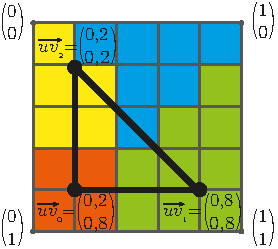
\includegraphics[width=0.43\textwidth]{img/texturierung/textur.pdf}
    \vspace{-10pt}
    \caption{Textur als 2D-Array mit uv-Koordinaten als Spaltenvektor der Form $ \binom{u}{v} \in \mathds{R}^2 $ }
    \label{fig:textur}
\end{wrapfigure}



In der Realität besitzen Objekte eine Vielzahl an geometrischen und materiellen Feinstrukturen. Beispiele dafür sind die Maserung bei Holz oder Kratzer und Unebenheiten in Oberflächen. Es wäre viel zu aufwendig, all diese Feinheiten durch ein polygonales Modell nachzubilden. Um Objekte dennoch mit solchen Details ausstatten zu können, verwendet die Computergrafik Texturen.

Abstrakt betrachtet, handelt es sich bei einer Textur um eine Funktion, die einen Punkt in der xy-Ebene auf ein Texturelement, auch Texel genannt, abbildet. Meistens werden Texturen durch Bitmaps realisiert. Diese bestehen aus einem 2D-Array in dem Farbwerte z.B. in RGB-Darstellung gespeichert werden. Daher werden Texel oft mit Farbwerten assoziiert. Tatsächlich können Texel auch andere Dinge repräsentieren wie z.B. Normalen oder Skalare. Dies hängt davon ab, wie Texturen umgesetzt werden und wie ein Texel interpretiert wird. Ein RGB-Farbwert besteht beispielsweise aus 3 Byte, wobei jedes Byte für einen der Farbkanäle Rot, Grün und Blau steht. Diese Bytes können jedoch auch als Komponenten einer Normalen verwendet werden.

Abb.~\ref{fig:textur} zeigt die schemenhafte Darstellung einer Bildtextur. Im Kontext der Texturierung heißen die Ebenenkoordinaten nicht wie üblich xy-Koordinaten sondern uv-Koordinaten. Diese sind meistens normiert und liegen deshalb im Intervall [0 1]. Um nun ein Objekt mit einer Textur zu überziehen, muss eine Abbildung der planaren uv-Koordinaten auf Punkte der Objektoberfläche stattfinden. Diese Abbildung wird auch "`Mapping"' genannt. Für einfache geometrische Objekte wie die Kugel kann die Mercator-Projektion verwendet werden, um die Kugeloberfläche auf eine Ebene zu projizieren und somit das Mapping der uv-Koordinaten durchzuführen. Für triangulierte Objekte wurde im Rahmen dieses Projekts die 3D-Modellierungssoftware "`3ds Max"' verwendet, um Dreiecksgitter auf eine Ebene zu projizieren und so mit Texturen zu versehen.

Abb.~\ref{fig:textur} zeigt ein Dreieck bei dem das "`Mapping"' bereits durchgeführt wurde. Jedem Dreieckspunkt ist eine der uv-Koordinaten \( \boldsymbol{uv_0}, \boldsymbol{uv_1} \text{ und } \boldsymbol{uv_2}\)  zugewiesen, wobei diese einen Spaltenvektor der Form \( \binom{u}{v} \in \mathds{R}^2 \) repräsentieren. Um nun die Färbung des Dreiecks an einem Schnittpunkt zu bestimmen, führt man den Dreiecksschnitttest durch, (s. Abschn.~\ref{sec:dreieck}) um die baryzentrischen Koordinaten \( \beta \text{ und } \gamma \) zu erhalten. Durch Interpolation der uv-Koordinaten lässt sich die Koordinate \( \boldsymbol{uv_r} \) am Schnittpunkt  bestimmen:

\begin{equation*}
    \boldsymbol{uv_r} = (1 - \beta - \gamma) \cdot \boldsymbol{uv_0} + \beta \cdot \boldsymbol{uv_1} + \gamma \cdot \boldsymbol{uv_2}
\end{equation*}

Die Komponenten von \( \boldsymbol{uv_r} \) können nun dazu benutzt werden, die entsprechenden Array-Indizes zu ermitteln, indem man \( u \) mit der Anzahl der Spalten und \( v \) mit der Anzahl der Zeilen des Arrays multipliziert (dazu müssen die uv-Koordinaten normalisiert sein).


\section{Normal Mapping}

\FloatBarrier


Neben der Möglichkeit, Objekte mit Farbinformationen zu versehen, können Texturen dazu verwendet werden, um Tiefeninformationen darzustellen, die in der Geometrie nicht vorhanden sind. Dazu können sogenannte "`Normal Maps"' verwendet werden. Sie werden typischerweise wie Farbtexturen als Bilder im RGB-Format gespeichert. Jedoch repräsentiert ein Texel keinen konkreten Farbwert, sondern wird als Vektor interpretiert, der dazu verwendet wird, die Ausrichtung der Oberflächennormalen zu verändern, wodurch ein Tiefeneindruck entsteht. Ziel dieser Vorgehensweise ist die Verkürzung von Rechenzeit, indem die Details eines komplexen Modells durch "`Normal Maps"' festgehalten und auf ein einfacheres Modell mit weniger Polygonen übertragen werden.

In Abb.~\ref{fig:trex_without_normalmap} wurde für die Bildsynthese das Modell eines T-Rex unter Verwendung glatter Schattierung (s. Abschn.~\ref{sec:facetierte_und_glatte_schattierung} ) verwendet. In Abb.~\ref{fig:trex_with_normalmap} ist das gleiche Modell unter Verwendung von "`Normal Mapping"' zu sehen.
Der einzige Unterschied besteht in der Ausrichtung der Oberflächennormalen, wodurch Falten und Vertiefungen vor allem an Kopf und Hals sichtbar werden, wobei die Rechenzeit nur geringfügig von 2,08 auf 2,1 Sekunden steigt.

\begin{minipage}[t]{0.45\textwidth}
   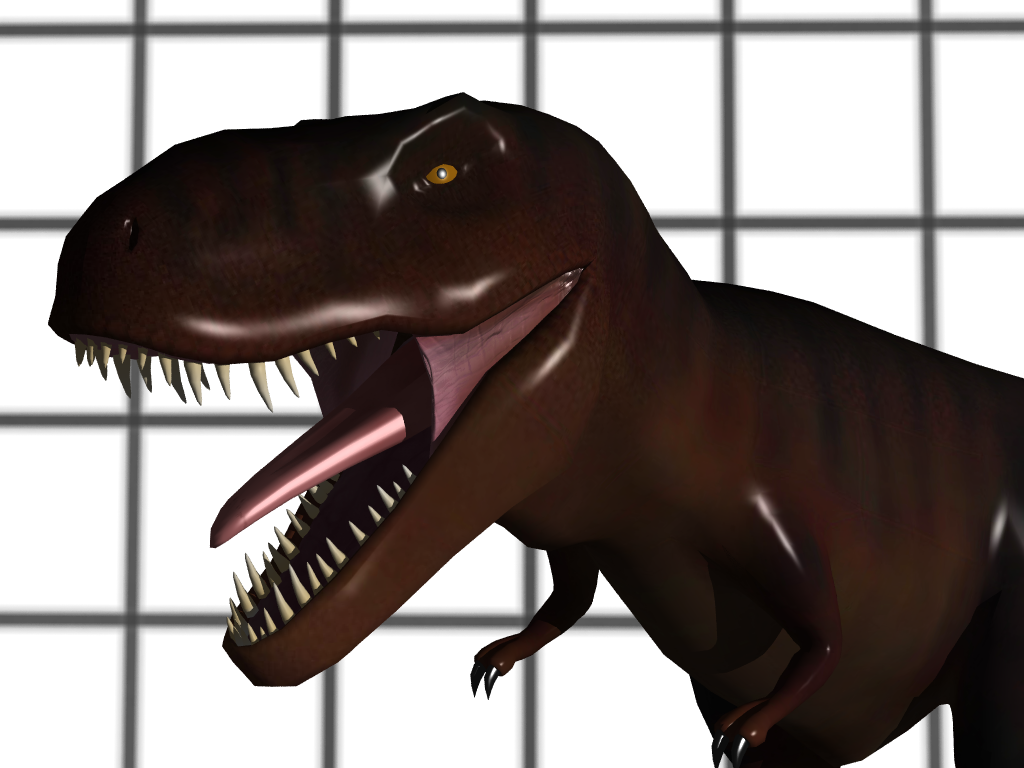
\includegraphics[width=\textwidth]{./img/texturierung/trex_without_normalmap}
   \captionof{figure}{Das Modell eines T-Rex ohne "`Normal Mapping"': Laufzeit 2,08 Sekunden}
   \label{fig:trex_without_normalmap}
\end{minipage}
   \hfill
\begin{minipage}[t]{0.45\textwidth}
   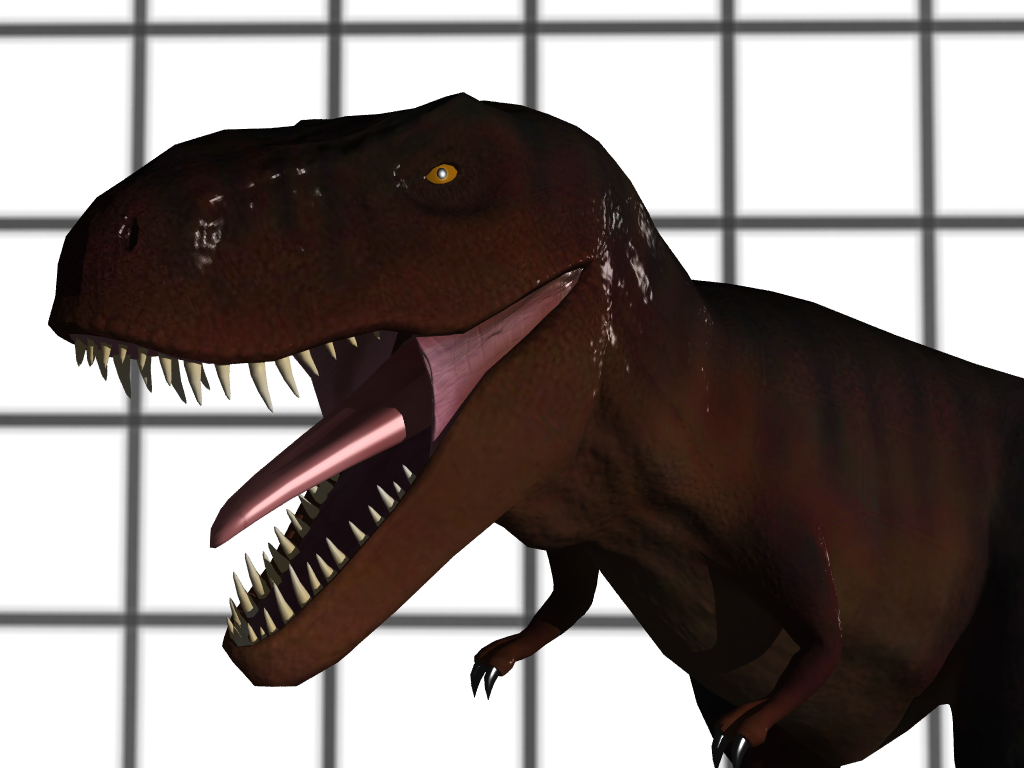
\includegraphics[width=\textwidth]{./img/texturierung/trex_with_normalmap}
   \captionof{figure}{Das selbe Modell mit "`Normal Mapping"': Laufzeit 2,1 Sekunden}
   \label{fig:trex_with_normalmap}
\end{minipage}

%\begin{figure}[t]
%    \centering
%    \begin{minipage}[b]{1.0\textwidth}
%        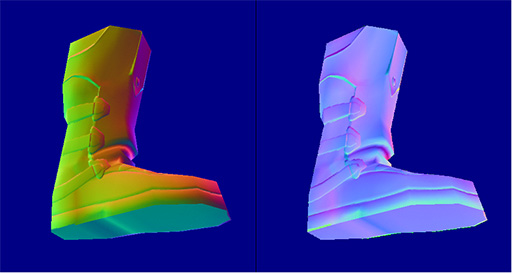
\includegraphics[width=\textwidth]{./img/texturierung/normalmaps}
%        \caption{Links: Regenbogenfarbene Objektraum-"'Normal Map"'. Rechts: Blaue Tangentialraum-"'Normal Map"'.\protect\footnotemark}
%        \label{Bild}
%    \end{minipage}
%\end{figure}

\begin{center}
    \begin{minipage}[t]{0.35\textwidth}
        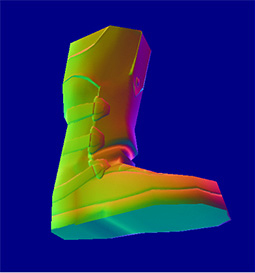
\includegraphics[width=\textwidth]{./img/texturierung/objektraum}
        \captionof{figure}{Objektraum-"'Normal Map"'\protect\footnotemark}
        \label{fig:objektraum}
    \end{minipage}
       \hspace{0.75cm}
       \addtocounter{footnote}{-1}\addtocounter{Hfootnote}{-1} % Setzt den Counter von footnotemark um 1 herunter
    \begin{minipage}[t]{0.35\textwidth}
       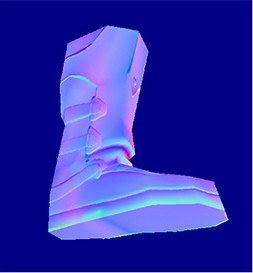
\includegraphics[width=\textwidth]{./img/texturierung/tangentialraum}
       \captionof{figure}{Tangentialraum-"'Normal Map"'\protect\footnotemark}
       \label{fig:tangentialraum}
   \end{minipage}
\end{center}
   
\footnotetext{Quelle: http://docs.cryengine.com/display/SDKDOC4/Tangent+Space+Normal+Mapping}

Man unterscheidet zwei Arten von "`Normal Maps"', die eine bezieht sich auf den Objektraum und die andere auf den Tangentialraum der Geometrie. In Abb.~\ref{fig:objektraum} sieht man, dass die Objektraum-"'Normal Map"' regenbogenfarben ausfällt. Dies liegt daran, dass die Objektraum-"'Normal Map"' Vektoren speichert, die direkt als Normalen an einem Oberflächenschnittpunkt benutzt werden können, solange das zugrunde liegende Objekt untransformiert bleibt. Gerade für geschlossene Polygonnetze entspricht das einer Verteilung der Normalen auf der Oberfläche einer Kugel, weshalb viele unterschiedliche Farben in der Textur zum Vorschein kommen.


Um nun für eine Objektraum-"'Normal Map"' die Normale an einem Schnittpunkt zu erhalten, sucht man den zum Schnittpunkt passenden Texel wie im vorherigen Abschnitt beschrieben. Die einzelnen Bytes des im Texel gespeicherten RBG-Werts sind dann \( r_{RGB} \) für Rot, \( g_{RGB} \) für Grün und \( b_{RGB} \) für Blau, wobei jede Komponente maximal den Wert 255 annehmen kann. Die Komponenten \( {n'}.x, {n'}.y \text{ und } {n'}.z \) der neuen variierten Normalen \( \boldsymbol{n'} \) ergeben sich dann durch:

\begin{equation}
    n'.x = \frac{2 \cdot r_{RGB} - r_{RGB}}{255}; \quad n'.y = \frac{2 \cdot g_{RGB} - g_{RGB}}{255}; \quad
    n'.z = \frac{2 \cdot b_{RGB} - b_{RGB}}{255}; \label{eq:texel_vektor}
\end{equation}

Wird das Objekt durch Transformationsmatrix \( \boldsymbol{T} \) transformiert, so muss die aus der Objektraum-"`Normal Map"' erhaltene Normale mit \( \boldsymbol{(T^{-1})}^\intercal \) transformiert werden.


Eine Tangentialraum-"'Normal Map"' (Abb.~\ref{fig:tangentialraum} ) bezieht sich hingegen auf die Koordinatenbasis, die durch einen Vektor senkrecht zur Oberfläche und zwei Tangentialvektoren gegeben ist. Der Ursprung der Basis befindet sich am Strahl-Objekt Schnittpunkt. Da auch bei unebenen Oberflächen die meisten Normalen relativ senkrecht auf der Oberfläche stehen und der Blauanteil der Textur für diese senkrechte (z-) Komponente verantwortlich ist, erscheint die Textur überwiegend bläulich.

Die Konstruktion der Koordinatenbasis beginnt mit der Festlegung der z-Achse. Dafür kann die beim Schnitttest berechnete Normale verwendet werden. Es ist jedoch auch möglich, eine interpolierte Normale zu benutzen, wie sie bei der glatten Schattierung verwendet wird, wodurch man harte Übergänge vermeidet.
Prinzipiell gibt es für die x- und y-Achse, die durch Tangentialvektoren festgelegt werden, beliebig viele Orientierungen, solange alle 3 Vektoren orthogonal zueinander stehen. Denn jede Drehung der x- und y-Achse um die z-Achse erzeugt weiterhin eine korrekte Koordinatenbasis im Tangentialraum. Für eine konsistente Schattierung ist es jedoch erforderlich, die Tangentialvektoren entlang der uv-Koordinaten auszurichten. Im Fall von triangulierten Objekten betrachtet man, wie sich die uv-Koordinaten entlang der Dreieckskanten verändern, indem man die Differenzen 
\( \Delta \boldsymbol{uv_0} = \boldsymbol{uv_1} - \boldsymbol{uv_0 }\) und \( \Delta \boldsymbol{uv_1} = \boldsymbol{uv_2} - \boldsymbol{uv_0} \) (vgl. Abb.\ref{fig:textur} ) bildet. Ebenso erzeugt man die Dreieckskanten \( \boldsymbol{e_0} = \boldsymbol{p_1} - \boldsymbol{p_0} \) und \( \boldsymbol{e_1} = \boldsymbol{p_2} - \boldsymbol{p_0} \), wobei  sich die uv-Koordinate \( \boldsymbol{uv_0} \) am Punkt \( \boldsymbol{p_0} \), \( \boldsymbol{uv_1} \) am Punkt \( \boldsymbol{p_1} \) usw. befindet.
Anhand der Komponenten von \( \Delta \boldsymbol{uv_0} \) und \( \Delta \boldsymbol{uv_1} \) wird eine Linearkombination mit den benötigten Basisvektoren d.h. mit der Tangenten \( \boldsymbol{t} \) und mit der Bitangenten \( \boldsymbol{b} \) gesucht, die den Kanten \( \boldsymbol{e_0} \) und \( \boldsymbol{e_1} \) entspricht \cite{openglnormal}:

\begin{align*}
    \boldsymbol{e_0} = {\Delta \boldsymbol{uv_0}.u } \cdot \boldsymbol{t} + {\Delta \boldsymbol{uv_0}.v } \cdot \boldsymbol{b} \\
    \boldsymbol{e_1} = {\Delta \boldsymbol{uv_1}.u } \cdot \boldsymbol{t} + {\Delta \boldsymbol{uv_1}.v } \cdot \boldsymbol{b}
\end{align*}

wobei \( {\Delta \boldsymbol{uv_0}.u } \) die \( u \)-Komponente von \( \Delta \boldsymbol{uv_0} \),  \( {\Delta \boldsymbol{uv_0}.v } \) die \( v \)-Komponente von \( \Delta \boldsymbol{uv_0} \) usw. ist.
Anhand dieses Gleichungssystems lässt sich nun \( \boldsymbol{t} \) und \( \boldsymbol{b} \) bestimmen, durch:

\begin{align*}
    r =& ({\Delta \boldsymbol{uv_0}.u } \cdot {\Delta \boldsymbol{uv_1}.v } - {\Delta \boldsymbol{uv_0}.v } \cdot {\Delta \boldsymbol{uv_1}.u } )^{-1} \\
    \boldsymbol{t} =& ( \boldsymbol{e_0} \cdot {\Delta \boldsymbol{uv_1}.v } - \boldsymbol{e_1} \cdot {\Delta \boldsymbol{uv_0}.v } ) \cdot r \\
    \boldsymbol{b} =& ( \boldsymbol{e_1} \cdot {\Delta \boldsymbol{uv_0}.u } - \boldsymbol{e_0} \cdot {\Delta \boldsymbol{uv_1}.u } ) \cdot r
\end{align*}

Die Vektoren \( \boldsymbol{t}, \boldsymbol{b} \text{ und } \boldsymbol{n} \) sind zwar linear unabhängig bilden jedoch keine ONB, weshalb das Gram-Schmidtsches Orthogonalisierungsverfahren eingesetzt wird, um diese Eigenschaft herzustellen. Zu beachten ist, dass dabei die Richtung von \( \boldsymbol{n} \) unverändert bleibt. Im Kontext des Verfahrens von Gram-Schmidt bedeutet das, dass man den Algorithmus mit dem Vektor \( \boldsymbol{n} \) beginnt.

Wie bei der Objektraum-"'Normal Map"' wird nun der zum Strahl-Objekt Schnittpunkt passende Texel gesucht und ein Vektor \( \boldsymbol{m} \)
gemäß der Gleichungen~\ref{eq:texel_vektor} erzeugt. Jedoch ist dies noch nicht die endgültige Normale \( \boldsymbol{n'} \). Diese erhält man durch:

\begin{equation*}
    \boldsymbol{n'} = \boldsymbol{t} \cdot {\boldsymbol{m}.x } + \boldsymbol{b} \cdot {\boldsymbol{m}.y } + \boldsymbol{n} \cdot  {\boldsymbol{m}.z }
\end{equation*}

wobei \( {\boldsymbol{m}.x }, {\boldsymbol{m}.y } \text{ und }  {\boldsymbol{m}.z } \) die x, y und z-Komponenten des Vektors \( \boldsymbol{m} \) sind.






